\chapter{PRÉ-PROCESSAMENTO}
\thispagestyle{plain}
\quad A captura do sinal de áudio é uma parte fundamental para o desenvolvimento de um sistema reconhecedor de fala. O som se propaga no ambiente por meio de ondas de forma contínua no tempo e no espaço a uma velocidade média de \textit{340 metros/segundo} fazendo  ar vibrar. Esta onda sonora  é capturada por meio de um microfone como uma onda analógia e  é convertida para um sinal digital. A onda capturada é normalizada através de um filtro de passa-baixas. Circuitos que realizam esta conversão de onda são chamados de  ADC (\textit{ analog digital converter}). O tamanho das amostras, expressa em bits, é um dos fatores que determina a precisão com que o som é representado em forma digital. Outro fator importante que afeta a qualidade de som é a taxa de amostragem. O teorema de Nyquist  afirma que a frequência mais elevada que pode ser representado com precisão é, no máximo, metade da taxa de amostragem \cite{nyqui}.

\section{Captura de Áudio}
\quad Para o processo de reconhecimento de fala de qualquer tipo, primeiro é necessário capturar o sinal de áudio. A fase de captura de áudio é essencial para o bom desempenho do projeto. Existem diversas bibliotecas open-source que oferecem funções que realizam a captura e gravação de áudio, entre elas a Allegro e OpenGL, entretanto a aplicação dessas bibliotecas implica em um maior custo computacional, uma vez que estas trazem milhares de linhas de código junto com outras funções além das necessárias para a implementação deste projeto. Com base nisso, buscou-se uma alternativa que integrasse eficiência e baixo custo computacional para aplicações em áudio. 
 
\subsection{ALSA}
\quad ALSA (\textit{advanced linux sound architeture }) consiste de um conjunto de drivers do kernel, uma biblioteca, uma API e programas utilitários para o suporte de som no linux. Jaroslav Kysela iniciou o projeto ALSA porque os drives de som do kernel Linux não estavam sendo devidamente mantidos e atualizados. Após  a iniciativa mais desenvolvedores aderiram ao projeto e a estrutura da API foi refinada. ALSA foi incorporada ao kernel oficial do Linux 2.5.
A biblioteca fornecida pelo ALSA, libasound, fornece uma nomeação lógica dos dispositivos de hardware. Os nomes podem ser de dispositivos de hardware reais ou plugins \cite{linux}. Os dispositivos de hardware usam o formato $HW:i,j$, onde $i$ é o número do cartão e $j$ do dispositivo do cartão. Uma placa de som tem um buffer de hardware que armazena amostras gravadas. Quando este buffer enche, ele gera uma interrupção. O driver de som do kernel, em seguida, utiliza o acesso direto à memória  para transferir as amostras para um buffer de aplicativo na memória. O tamanho deste buffer pode ser  programado por chamadas da biblioteca ALSA. Caso o buffer seja muito grande a tranferencia geraria uma latência excessiva. ALSA resolve isso dividindo o buffer em fragmentos e transfere os dados fragmentados. A Figura \ref{fig:pcm} ilustra a repartição do buffer em fragmentos, molduras e amostras.

\begin{figure}[H]
\centering % para centralizarmos a figura
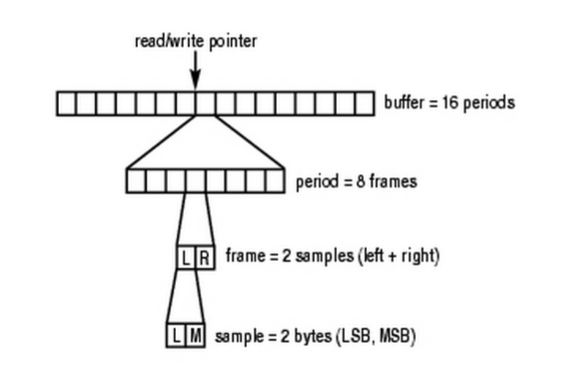
\includegraphics[width=10cm]{img/pcm.jpg} % leia abaixo
\caption{Buffer de aplicação. \textit{fonte:\cite{linux}}}
\label{fig:pcm}
\end{figure}

\quad A API ALSA oferece seis principais interfaces. São elas  a interface de controle, interface MIDI raw, interface de tempo, interface de sequência, interface mixer e interface de PCM. Esta última gerencia a captura e reprodução de áudio digital. 


\section{Arquivos WAVE}

\quad O formato de áudio adotado foi o WAVE. Neste tipo de formato o som é armazenado em sequências numéricas. O áudio é convertido em dados e armazenado bit a bit. O WAVE (.wav) foi criado pela IBM e pela Microsoft, nos anos oitenta e tem suporte a  uma série de resoluções de bit, taxas de amostragens e canais de áudio.  A taxa de amostragem em arquivo .wav refere-se ao número de amostras por segundo. O CD possui uma taxa de amsotragem de $44,100$, o que significa que cada segundo de áudio tem $44,100$ amostras. A quantidade de bits usada determina  quanta informação pode ser armazenada  no arquivo. A quantidade de bits também interfere na amplitude do sinal. Em uma gravação de 8 bits estará disponível 256 níveis de amplitude, variando de $0$ à $255$. Em uma gravação de 16 bits a quantidade de níveis de amplitude disponíveis passa a $65,536$, variando entre $-32,768$  até $32767$. A quantidade de 16 bits é suficiente para este projeto. 

\subsection{Cabeçalho WAVE}

\quad O cabeçalho de um arquivo .wav possui 44 bytes e é organizado como mostrado na Tabela \ref{tab:app}.

\begin{table}[H]
\centering
\caption{Formato de um cabeçalho de arquivo wave}
\label{tab:app}
\smallskip
\begin{tabular}{|l|l|l|}
\hline
Posição & Valor & Descrição\\[0.5ex]
\hline
&&\\[-2ex]
1 - 4& RIFF & Define como um arquivo RIFF \\[0.5ex]
\hline
&&\\[-2ex]
5 - 8& Tamanho do arquivo (int) & Tamanho máximo do arquivos em bytes \\[0.5ex]
\hline
&&\\[-2ex]
9 - 12 & "WAVE" & Arquivo tipo cabeçalho wave\\[0.5ex]
\hline
&&\\[-2ex]
13 - 16& "fmt" & Marca formato chunk \\[0.5ex]
\hline
&&\\[-2ex]
17 - 20& 16& Tamanho do formato dos dados \\[0.5ex]
\hline
&&\\[-2ex]
21 - 22& 1& Formato tipo PCM\\[0.5ex]
\hline
&&\\[-2ex]
23 - 24& 2 & Quantidade de canais\\[0.5ex]
\hline
&&\\[-2ex]
25 - 28& 44100 & Taxa de amostragem (sample rate) \\[0.5ex]
\hline
&&\\[-2ex]
29 - 32& 176400& (sample rate * bitspersample * channels) / 8 \\[0.5ex]
\hline
&&\\[-2ex]
33 - 34&  4 & limites \\[0.5ex]
\hline
&&\\[-2ex]
35 - 36& 16 & Quantidade de bits por amostra \\[0.5ex]
\hline
&&\\[-2ex]
37 - 40& data & Marca o início da seção de dados \\[0.5ex]
\hline
&&\\[-2ex]
41 - 44& Tamanho do arquivo (dados) & Tamanho da seção de dados \\[0.5ex]
\hline
\end{tabular}
\end{table}



